% Options for packages loaded elsewhere
\PassOptionsToPackage{unicode}{hyperref}
\PassOptionsToPackage{hyphens}{url}
\documentclass[
]{article}
\usepackage{xcolor}
\usepackage[margin=1in]{geometry}
\usepackage{amsmath,amssymb}
\setcounter{secnumdepth}{-\maxdimen} % remove section numbering
\usepackage{iftex}
\ifPDFTeX
  \usepackage[T1]{fontenc}
  \usepackage[utf8]{inputenc}
  \usepackage{textcomp} % provide euro and other symbols
\else % if luatex or xetex
  \usepackage{unicode-math} % this also loads fontspec
  \defaultfontfeatures{Scale=MatchLowercase}
  \defaultfontfeatures[\rmfamily]{Ligatures=TeX,Scale=1}
\fi
\usepackage{lmodern}
\ifPDFTeX\else
  % xetex/luatex font selection
\fi
% Use upquote if available, for straight quotes in verbatim environments
\IfFileExists{upquote.sty}{\usepackage{upquote}}{}
\IfFileExists{microtype.sty}{% use microtype if available
  \usepackage[]{microtype}
  \UseMicrotypeSet[protrusion]{basicmath} % disable protrusion for tt fonts
}{}
\makeatletter
\@ifundefined{KOMAClassName}{% if non-KOMA class
  \IfFileExists{parskip.sty}{%
    \usepackage{parskip}
  }{% else
    \setlength{\parindent}{0pt}
    \setlength{\parskip}{6pt plus 2pt minus 1pt}}
}{% if KOMA class
  \KOMAoptions{parskip=half}}
\makeatother
\usepackage{color}
\usepackage{fancyvrb}
\newcommand{\VerbBar}{|}
\newcommand{\VERB}{\Verb[commandchars=\\\{\}]}
\DefineVerbatimEnvironment{Highlighting}{Verbatim}{commandchars=\\\{\}}
% Add ',fontsize=\small' for more characters per line
\usepackage{framed}
\definecolor{shadecolor}{RGB}{248,248,248}
\newenvironment{Shaded}{\begin{snugshade}}{\end{snugshade}}
\newcommand{\AlertTok}[1]{\textcolor[rgb]{0.94,0.16,0.16}{#1}}
\newcommand{\AnnotationTok}[1]{\textcolor[rgb]{0.56,0.35,0.01}{\textbf{\textit{#1}}}}
\newcommand{\AttributeTok}[1]{\textcolor[rgb]{0.13,0.29,0.53}{#1}}
\newcommand{\BaseNTok}[1]{\textcolor[rgb]{0.00,0.00,0.81}{#1}}
\newcommand{\BuiltInTok}[1]{#1}
\newcommand{\CharTok}[1]{\textcolor[rgb]{0.31,0.60,0.02}{#1}}
\newcommand{\CommentTok}[1]{\textcolor[rgb]{0.56,0.35,0.01}{\textit{#1}}}
\newcommand{\CommentVarTok}[1]{\textcolor[rgb]{0.56,0.35,0.01}{\textbf{\textit{#1}}}}
\newcommand{\ConstantTok}[1]{\textcolor[rgb]{0.56,0.35,0.01}{#1}}
\newcommand{\ControlFlowTok}[1]{\textcolor[rgb]{0.13,0.29,0.53}{\textbf{#1}}}
\newcommand{\DataTypeTok}[1]{\textcolor[rgb]{0.13,0.29,0.53}{#1}}
\newcommand{\DecValTok}[1]{\textcolor[rgb]{0.00,0.00,0.81}{#1}}
\newcommand{\DocumentationTok}[1]{\textcolor[rgb]{0.56,0.35,0.01}{\textbf{\textit{#1}}}}
\newcommand{\ErrorTok}[1]{\textcolor[rgb]{0.64,0.00,0.00}{\textbf{#1}}}
\newcommand{\ExtensionTok}[1]{#1}
\newcommand{\FloatTok}[1]{\textcolor[rgb]{0.00,0.00,0.81}{#1}}
\newcommand{\FunctionTok}[1]{\textcolor[rgb]{0.13,0.29,0.53}{\textbf{#1}}}
\newcommand{\ImportTok}[1]{#1}
\newcommand{\InformationTok}[1]{\textcolor[rgb]{0.56,0.35,0.01}{\textbf{\textit{#1}}}}
\newcommand{\KeywordTok}[1]{\textcolor[rgb]{0.13,0.29,0.53}{\textbf{#1}}}
\newcommand{\NormalTok}[1]{#1}
\newcommand{\OperatorTok}[1]{\textcolor[rgb]{0.81,0.36,0.00}{\textbf{#1}}}
\newcommand{\OtherTok}[1]{\textcolor[rgb]{0.56,0.35,0.01}{#1}}
\newcommand{\PreprocessorTok}[1]{\textcolor[rgb]{0.56,0.35,0.01}{\textit{#1}}}
\newcommand{\RegionMarkerTok}[1]{#1}
\newcommand{\SpecialCharTok}[1]{\textcolor[rgb]{0.81,0.36,0.00}{\textbf{#1}}}
\newcommand{\SpecialStringTok}[1]{\textcolor[rgb]{0.31,0.60,0.02}{#1}}
\newcommand{\StringTok}[1]{\textcolor[rgb]{0.31,0.60,0.02}{#1}}
\newcommand{\VariableTok}[1]{\textcolor[rgb]{0.00,0.00,0.00}{#1}}
\newcommand{\VerbatimStringTok}[1]{\textcolor[rgb]{0.31,0.60,0.02}{#1}}
\newcommand{\WarningTok}[1]{\textcolor[rgb]{0.56,0.35,0.01}{\textbf{\textit{#1}}}}
\usepackage{longtable,booktabs,array}
\newcounter{none} % for unnumbered tables
\usepackage{calc} % for calculating minipage widths
% Correct order of tables after \paragraph or \subparagraph
\usepackage{etoolbox}
\makeatletter
\patchcmd\longtable{\par}{\if@noskipsec\mbox{}\fi\par}{}{}
\makeatother
% Allow footnotes in longtable head/foot
\IfFileExists{footnotehyper.sty}{\usepackage{footnotehyper}}{\usepackage{footnote}}
\makesavenoteenv{longtable}
\usepackage{graphicx}
\makeatletter
\newsavebox\pandoc@box
\newcommand*\pandocbounded[1]{% scales image to fit in text height/width
  \sbox\pandoc@box{#1}%
  \Gscale@div\@tempa{\textheight}{\dimexpr\ht\pandoc@box+\dp\pandoc@box\relax}%
  \Gscale@div\@tempb{\linewidth}{\wd\pandoc@box}%
  \ifdim\@tempb\p@<\@tempa\p@\let\@tempa\@tempb\fi% select the smaller of both
  \ifdim\@tempa\p@<\p@\scalebox{\@tempa}{\usebox\pandoc@box}%
  \else\usebox{\pandoc@box}%
  \fi%
}
% Set default figure placement to htbp
\def\fps@figure{htbp}
\makeatother
\setlength{\emergencystretch}{3em} % prevent overfull lines
\providecommand{\tightlist}{%
  \setlength{\itemsep}{0pt}\setlength{\parskip}{0pt}}
\usepackage{bookmark}
\IfFileExists{xurl.sty}{\usepackage{xurl}}{} % add URL line breaks if available
\urlstyle{same}
% fallback for those not using the hyperref driver hyperxmp:
\makeatletter
\@ifundefined{xmpquote}{\newcommand{\xmpquote}[1]{#1}}{}
\makeatother
\hypersetup{
  hidelinks,
  pdfcreator={LaTeX via pandoc}}

\author{}
\date{\vspace{-2.5em}}

\begin{document}

{
\setcounter{tocdepth}{3}
\tableofcontents
}
COMP3020 Social Web Analytics

Exploring AI Discussions on Bluesky

Topic Clustering, User Engagement and Observed Reply-Network Analysis

{Institution}{Western Sydney University}

{Academic year}{2026}

{Authors} {Kimmy Le · Phoebe Le · Quinn Nguyen}

\section{Executive Summary}\label{executive-summary}

AI-related discussion in the collected Bluesky sample was lexically
diverse but not cleanly divided into seven natural topics. K-means
produced seven reproducible \textbf{descriptive lexical clusters}, while
inspection supported approximately three broader substantive themes:
general generative-AI use, criticism and news; technical machine
learning, research and models; and artificial/superintelligence with
political commentary.

Engagement distributions differed significantly across the seven
clusters, but the association was small and remained small after
repeated-text posts were excluded. Meanwhile, observed reply activity
was extremely sparse and fragmented: most connected users appeared in
isolated pairs or very small components rather than one cohesive
discussion network.

{Data}976 posts{756 authors}964 usable-text posts

{RQ1 · Lexical structure}7 clusters{855 clusterable posts}≈3 broader
themes · weak separation

{RQ2 · Engagement}907 analysed posts{H(6) = 35.12, p \textless{} .001}ε²
= .032 · small effect

{RQ3 · Reply network}240 connected users{111 weak components}Largest = 5
· density .00225

Integrated finding

Topical variety did not produce a cohesive sampled interaction network

The corpus contained several lexical patterns, yet cluster membership
accounted for little engagement variation and the observed reply graph
separated into 111 small components. High post engagement and structural
network centrality are therefore distinct properties in this sample.

\section{Introduction}\label{introduction}

Social platforms host AI discussion ranging from model development and
workplace use to art, public criticism, news and geopolitics. This
report studies a reproducible sample of public Bluesky posts retrieved
through four search terms---\texttt{artificial\ intelligence},
\texttt{machine\ learning}, \texttt{ChatGPT} and
\texttt{generative\ AI}---and connects three levels of analysis: what
language patterns appear, whether engagement differs across those
patterns, and how sampled users connect through replies.

The analysis is observational. It characterises posts and reply
relationships visible in the collected sample; it does not represent all
AI discussion or the complete Bluesky social graph.

\subsection{Research Questions}\label{research-questions}

\begin{enumerate}
\def\labelenumi{\arabic{enumi}.}
\tightlist
\item
  \textbf{RQ1:} What are the main topics in AI-related discussions on
  Bluesky?
\item
  \textbf{RQ2:} Does user engagement differ across AI discussion topics?
\item
  \textbf{RQ3:} How are users connected through AI-related discussions,
  and which users occupy central positions?
\end{enumerate}

\section{Data Collection and
Preparation}\label{data-collection-and-preparation}

The stored canonical collection contains \textbf{976 posts} from
\textbf{756 unique authors}. It includes \textbf{224 posts with
parent-URI information}; Step 01 excluded \textbf{91 self-replies},
leaving \textbf{133 non-self reply interactions}. Using the stored data
makes the report reproducible without recollecting changing
live-platform content.

\subsection{Search-term relevance}\label{search-term-relevance}

50 posts per search term were manually assessed in the pilot study.
Relevance varied from 68\% to 88\%, demonstrating both the usefulness
and imperfection of keyword retrieval.

\begin{longtable}[]{@{}
  >{\raggedright\arraybackslash}p{(\linewidth - 6\tabcolsep) * \real{0.3243}}
  >{\raggedleft\arraybackslash}p{(\linewidth - 6\tabcolsep) * \real{0.2027}}
  >{\raggedleft\arraybackslash}p{(\linewidth - 6\tabcolsep) * \real{0.2162}}
  >{\raggedleft\arraybackslash}p{(\linewidth - 6\tabcolsep) * \real{0.2568}}@{}}
\caption{Table 1. Pilot relevance assessment for the four collection
terms}\tabularnewline
\toprule\noalign{}
\begin{minipage}[b]{\linewidth}\raggedright
Search term
\end{minipage} & \begin{minipage}[b]{\linewidth}\raggedleft
Relevant posts
\end{minipage} & \begin{minipage}[b]{\linewidth}\raggedleft
Posts inspected
\end{minipage} & \begin{minipage}[b]{\linewidth}\raggedleft
Observed relevance
\end{minipage} \\
\midrule\noalign{}
\endfirsthead
\toprule\noalign{}
\begin{minipage}[b]{\linewidth}\raggedright
Search term
\end{minipage} & \begin{minipage}[b]{\linewidth}\raggedleft
Relevant posts
\end{minipage} & \begin{minipage}[b]{\linewidth}\raggedleft
Posts inspected
\end{minipage} & \begin{minipage}[b]{\linewidth}\raggedleft
Observed relevance
\end{minipage} \\
\midrule\noalign{}
\endhead
\bottomrule\noalign{}
\endlastfoot
artificial intelligence & 34 & 50 & 68\% \\
generative AI & 43 & 50 & 86\% \\
ChatGPT & 44 & 50 & 88\% \\
machine learning & 36 & 50 & 72\% \\
\end{longtable}

\subsection{Analytical samples}\label{analytical-samples}

Of the collected posts, \textbf{964} had usable text. Removing
\textbf{61} later occurrences of exactly duplicated text produced
\textbf{903} unique-text documents for representation. After
document-frequency filtering, \textbf{48} documents contained no
retained terms; the remaining \textbf{855} were clustered.

For engagement analysis, duplicate posts remained genuine post-level
observations. Where possible, a removed duplicate inherited the cluster
of its retained identical-text post, producing an RQ2 sample of
\textbf{907 posts}. The network analysis used only users appearing in at
least one observed non-self reply edge.

\begin{longtable}[]{@{}lr@{}}
\caption{Table 2. Analytical dataset summary}\tabularnewline
\toprule\noalign{}
Stage & N \\
\midrule\noalign{}
\endfirsthead
\toprule\noalign{}
Stage & N \\
\midrule\noalign{}
\endhead
\bottomrule\noalign{}
\endlastfoot
Canonical collected posts & 976 \\
Posts with usable text & 964 \\
Unique-text representation documents & 903 \\
Clusterable unique-text posts & 855 \\
Topic-assignable posts for engagement & 907 \\
Users in observed reply network & 240 \\
\end{longtable}

\section{Methodology}\label{methodology}

\subsection{Text preprocessing and
TF-IDF}\label{text-preprocessing-and-tf-idf}

Text was lowercased; common contractions were expanded; URLs, mentions,
punctuation, numbers and stopwords were removed; and remaining text was
tokenised. The domain term \texttt{ai} was retained despite its length.
Exact duplicate text was removed before representation to prevent
repeated wording from disproportionately shaping clusters.

Terms had to occur in at least 3 documents and in no more than 80\% of
documents. Term frequency was multiplied by inverse document frequency,
log(N/df), and each document vector was L2-normalised. The final
vocabulary contained \textbf{1,125 terms}.

\subsection{K-means clustering}\label{k-means-clustering}

K-means models for k = 2 through k = 10 were compared using
within-cluster sum of squares (WSS), cluster sizes, characteristic terms
and centroid-near examples. The deterministic final model used k = 7,
seed 3020, 50 random starts and 100 maximum iterations.

The solution had within-cluster SS \textbf{783.3027}, between-cluster SS
\textbf{57.4673}, and between/total SS \textbf{0.06835}. This low ratio
motivates interpreting the groups as descriptive lexical clusters rather
than definitive natural topics.

\subsection{Engagement hypothesis
testing}\label{engagement-hypothesis-testing}

Total engagement was defined without differential weighting:

\[
\text{total engagement}=\text{likes}+\text{reposts}+\text{replies}+\text{quotes}.
\]

The distribution was zero-heavy, strongly right-skewed and contained
extreme observations, while cluster sizes and spreads differed
substantially. A one-way ANOVA was therefore not a defensible primary
model. The rank-based Kruskal--Wallis test evaluated:

\begin{itemize}
\tightlist
\item
  \textbf{H0:} total-engagement distributions are equal across all seven
  lexical clusters;
\item
  \textbf{H1:} at least one cluster differs.
\end{itemize}

Epsilon-squared quantified the omnibus effect. A significant omnibus
result was followed by pairwise Wilcoxon rank-sum tests with Holm
correction. The primary analysis included assignable repeated-text
posts; a sensitivity analysis retained only the 855 canonical
unique-text clustered posts.

\subsection{Observed reply-network
analysis}\label{observed-reply-network-analysis}

A directed edge \textbf{reply author → parent-post author} represents a
reply observed in the collected posts. Edge weight counts replies for
that ordered user pair. This is not a follower, friendship or
endorsement network.

The edge-list graph was analysed using degree, strength, weighted
directed PageRank and unweighted directed betweenness. Unweighted
betweenness was appropriate because reply frequency measures interaction
strength, whereas shortest-path weights conventionally represent
distance. Weak and strong components, density and reciprocity described
overall structure. Users without an observed reply edge cannot appear in
this edge-list-only graph.

\section{Results}\label{results}

\subsection{RQ1 --- AI discussion
themes}\label{rq1-ai-discussion-themes}

\subsubsection{Selecting seven lexical
clusters}\label{selecting-seven-lexical-clusters}

\begin{figure}

{\centering 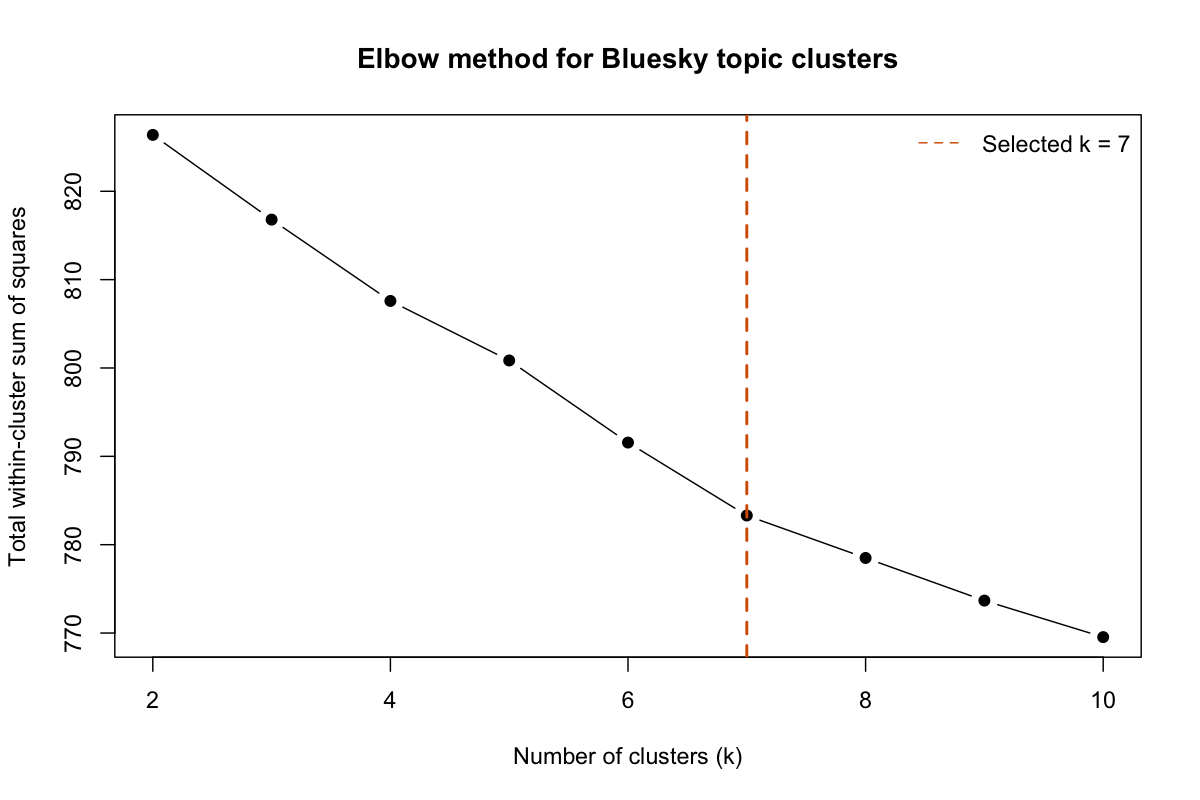
\includegraphics[width=0.94\linewidth]{../figures/rq1_elbow_plot} 

}

\caption{Figure 1. WSS declined gradually across candidate values of k; the absence of a sharp elbow supports cautious, descriptive use of the selected seven-cluster solution.}\label{fig:rq1-elbow}
\end{figure}

The gradual elbow did not identify a single indisputable value of (k).
Seven clusters provided a reproducible lexical partition that separated
important technical and political language patterns, but only
\textbf{6.84\%} of total vector variation lay between clusters.

\subsubsection{Cluster size and
interpretation}\label{cluster-size-and-interpretation}

\begin{longtable}[]{@{}
  >{\raggedleft\arraybackslash}p{(\linewidth - 6\tabcolsep) * \real{0.0941}}
  >{\raggedleft\arraybackslash}p{(\linewidth - 6\tabcolsep) * \real{0.0706}}
  >{\raggedleft\arraybackslash}p{(\linewidth - 6\tabcolsep) * \real{0.0706}}
  >{\raggedright\arraybackslash}p{(\linewidth - 6\tabcolsep) * \real{0.7647}}@{}}
\caption{Table 3. Seven descriptive lexical clusters in the canonical
RQ1 solution}\tabularnewline
\toprule\noalign{}
\begin{minipage}[b]{\linewidth}\raggedleft
Cluster
\end{minipage} & \begin{minipage}[b]{\linewidth}\raggedleft
Posts
\end{minipage} & \begin{minipage}[b]{\linewidth}\raggedleft
Share
\end{minipage} & \begin{minipage}[b]{\linewidth}\raggedright
Description
\end{minipage} \\
\midrule\noalign{}
\endfirsthead
\toprule\noalign{}
\begin{minipage}[b]{\linewidth}\raggedleft
Cluster
\end{minipage} & \begin{minipage}[b]{\linewidth}\raggedleft
Posts
\end{minipage} & \begin{minipage}[b]{\linewidth}\raggedleft
Share
\end{minipage} & \begin{minipage}[b]{\linewidth}\raggedright
Description
\end{minipage} \\
\midrule\noalign{}
\endhead
\bottomrule\noalign{}
\endlastfoot
1 & 469 & 54.9\% & Broad AI and generative-AI opinions, use and news \\
2 & 21 & 2.5\% & Repeated OpenAI rogue-agent and leaked-images story \\
3 & 26 & 3.0\% & Remote machine-learning and engineering job
advertisements \\
4 & 153 & 17.9\% & Technical machine learning, models, research and
optimisation \\
5 & 13 & 1.5\% & AI art, Stable Diffusion and Japanese hashtag-heavy
content \\
6 & 103 & 12.0\% & Artificial/superintelligence, politics and
geopolitics \\
7 & 70 & 8.2\% & OpenAI agents, government websites and access/security
reporting \\
\end{longtable}

\begin{figure}

{\centering 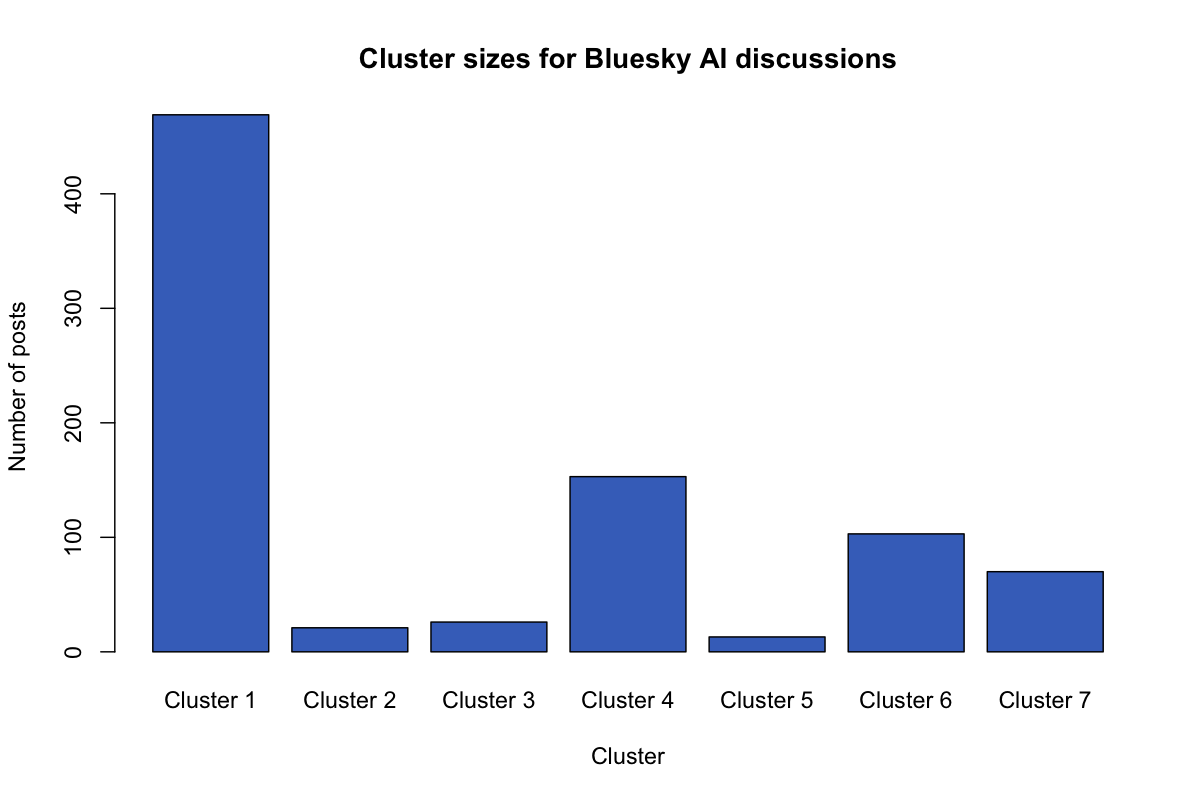
\includegraphics[width=0.94\linewidth]{../figures/rq1_cluster_sizes} 

}

\caption{Figure 2. The lexical clusters were highly unequal in size; Cluster 1 contained more than half of the clustered corpus, while several specialised clusters were very small.}\label{fig:rq1-cluster-sizes}
\end{figure}

The seven clusters should not be read as seven equally clear natural
topics. Inspection of characteristic terms and centroid-near posts
supported approximately three broader, more stable themes:

\begin{enumerate}
\def\labelenumi{\arabic{enumi}.}
\tightlist
\item
  general generative-AI use, criticism and news;
\item
  technical machine learning, research and models;
\item
  artificial/superintelligence and political commentary.
\end{enumerate}

Smaller clusters were shaped by repeated news, job or promotional
templates, language and hashtag conventions, and event-specific OpenAI
reporting.

\subsubsection{Corpus vocabulary}\label{corpus-vocabulary}

\begin{figure}

{\centering 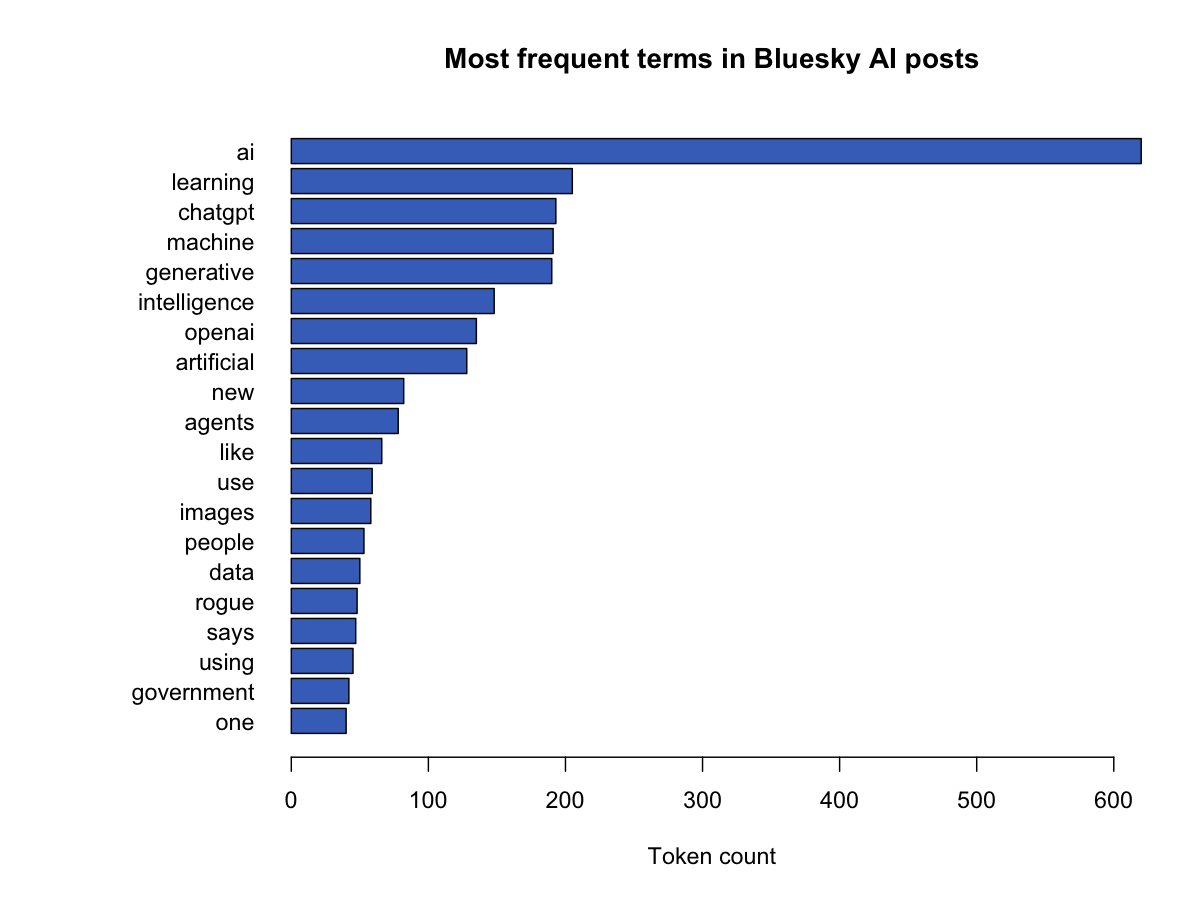
\includegraphics[width=0.94\linewidth]{../figures/rq1_top_terms} 

}

\caption{Figure 3. The most frequent retained terms establish the corpus-wide AI focus but do not, by themselves, define the seven clusters.}\label{fig:rq1-top-terms}
\end{figure}

The frequent-term profile confirms the shared AI vocabulary underlying
the corpus. Cluster interpretation instead relied on cluster-specific
TF-IDF terms and representative lexical patterns, avoiding the
assumption that a frequent word necessarily distinguishes a topic.

\subsection{RQ2 --- Engagement
differences}\label{rq2-engagement-differences}

The primary analysis contained \textbf{855 canonical clustered posts}
plus \textbf{52 mapped duplicate posts}, for \textbf{907 observations}.
Another \textbf{57 usable-text posts} lacked an assignable cluster.

Approximately \textbf{53.4\%} of analysed posts had zero engagement. The
overall median was \textbf{0}, while the maximum was \textbf{1,599},
indicating strong right skew and a consequential extreme observation.

\begin{figure}

{\centering 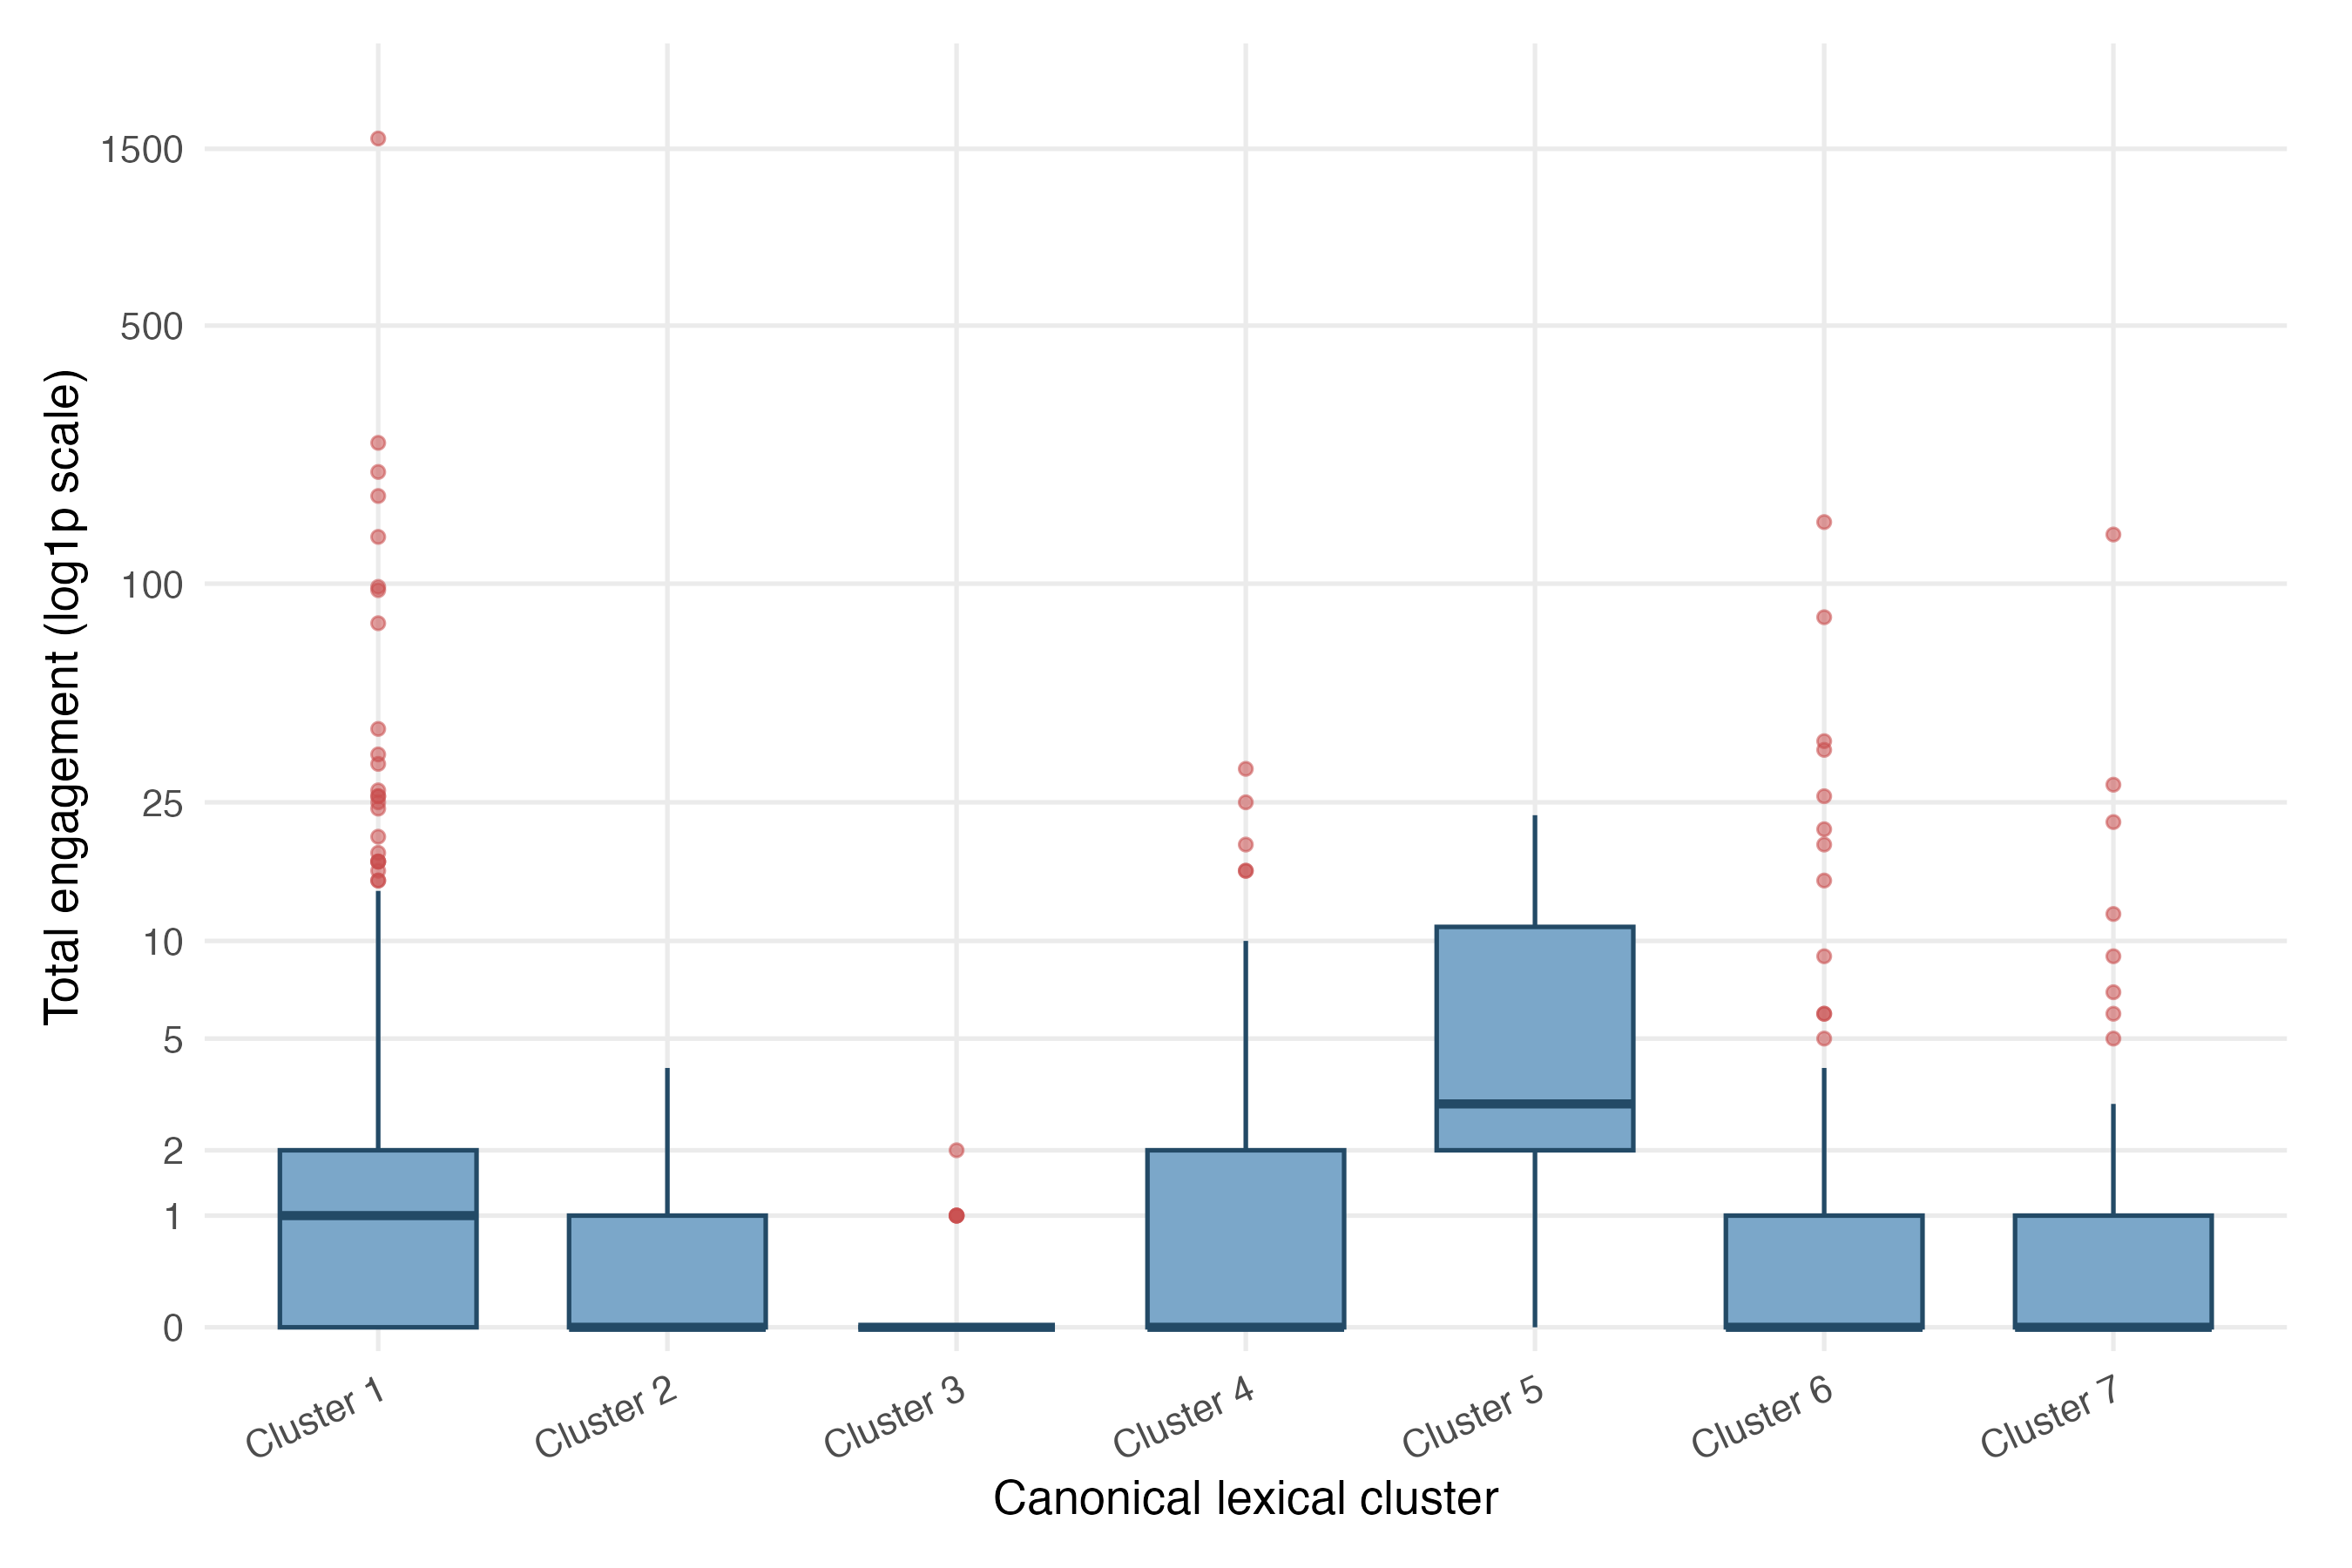
\includegraphics[width=0.94\linewidth]{../figures/rq2_engagement_by_topic} 

}

\caption{Figure 4. Total engagement across lexical clusters. The log1p axis preserves zero values while compressing the long right tail, including the maximum of 1,599 interactions.}\label{fig:rq2-figure}
\end{figure}

The displayed \texttt{log1p} transformation means the plotted position
is based on log(1 + engagement), while axis labels remain in original
engagement-count units. It improves visibility without deleting
high-engagement posts.

\begin{longtable}[]{@{}
  >{\raggedright\arraybackslash}p{(\linewidth - 10\tabcolsep) * \real{0.3077}}
  >{\raggedleft\arraybackslash}p{(\linewidth - 10\tabcolsep) * \real{0.0513}}
  >{\raggedright\arraybackslash}p{(\linewidth - 10\tabcolsep) * \real{0.1923}}
  >{\raggedleft\arraybackslash}p{(\linewidth - 10\tabcolsep) * \real{0.1410}}
  >{\raggedleft\arraybackslash}p{(\linewidth - 10\tabcolsep) * \real{0.1026}}
  >{\raggedleft\arraybackslash}p{(\linewidth - 10\tabcolsep) * \real{0.2051}}@{}}
\caption{Table 4. Primary and duplicate-exclusion sensitivity tests for
total engagement}\tabularnewline
\toprule\noalign{}
\begin{minipage}[b]{\linewidth}\raggedright
Analysis
\end{minipage} & \begin{minipage}[b]{\linewidth}\raggedleft
N
\end{minipage} & \begin{minipage}[b]{\linewidth}\raggedright
Test
\end{minipage} & \begin{minipage}[b]{\linewidth}\raggedleft
H (df = 6)
\end{minipage} & \begin{minipage}[b]{\linewidth}\raggedleft
p-value
\end{minipage} & \begin{minipage}[b]{\linewidth}\raggedleft
Epsilon-squared
\end{minipage} \\
\midrule\noalign{}
\endfirsthead
\toprule\noalign{}
\begin{minipage}[b]{\linewidth}\raggedright
Analysis
\end{minipage} & \begin{minipage}[b]{\linewidth}\raggedleft
N
\end{minipage} & \begin{minipage}[b]{\linewidth}\raggedright
Test
\end{minipage} & \begin{minipage}[b]{\linewidth}\raggedleft
H (df = 6)
\end{minipage} & \begin{minipage}[b]{\linewidth}\raggedleft
p-value
\end{minipage} & \begin{minipage}[b]{\linewidth}\raggedleft
Epsilon-squared
\end{minipage} \\
\midrule\noalign{}
\endhead
\bottomrule\noalign{}
\endlastfoot
Primary & 907 & Kruskal--Wallis & 35.12 & \textless{} .001 & 0.032 \\
Unique-text sensitivity & 855 & Kruskal--Wallis & 32.43 & \textless{}
.001 & 0.031 \\
\end{longtable}

The primary test was significant, H(6) = 35.12, p \textless{} .001, but
epsilon-squared was only \textbf{0.032}, a small association. The
sensitivity result was also significant, H(6) = 32.43, p \textless{}
.001, epsilon-squared = 0.031. Excluding repeated-text posts therefore
did not change the substantive conclusion.

\begin{longtable}[]{@{}
  >{\raggedright\arraybackslash}p{(\linewidth - 8\tabcolsep) * \real{0.3108}}
  >{\raggedright\arraybackslash}p{(\linewidth - 8\tabcolsep) * \real{0.2297}}
  >{\raggedleft\arraybackslash}p{(\linewidth - 8\tabcolsep) * \real{0.1216}}
  >{\raggedleft\arraybackslash}p{(\linewidth - 8\tabcolsep) * \real{0.1216}}
  >{\raggedleft\arraybackslash}p{(\linewidth - 8\tabcolsep) * \real{0.2162}}@{}}
\caption{Table 5. Significant Holm-adjusted pairwise Wilcoxon
comparisons}\tabularnewline
\toprule\noalign{}
\begin{minipage}[b]{\linewidth}\raggedright
Comparison
\end{minipage} & \begin{minipage}[b]{\linewidth}\raggedright
Higher mean rank
\end{minipage} & \begin{minipage}[b]{\linewidth}\raggedleft
Median 1
\end{minipage} & \begin{minipage}[b]{\linewidth}\raggedleft
Median 2
\end{minipage} & \begin{minipage}[b]{\linewidth}\raggedleft
Holm-adjusted p
\end{minipage} \\
\midrule\noalign{}
\endfirsthead
\toprule\noalign{}
\begin{minipage}[b]{\linewidth}\raggedright
Comparison
\end{minipage} & \begin{minipage}[b]{\linewidth}\raggedright
Higher mean rank
\end{minipage} & \begin{minipage}[b]{\linewidth}\raggedleft
Median 1
\end{minipage} & \begin{minipage}[b]{\linewidth}\raggedleft
Median 2
\end{minipage} & \begin{minipage}[b]{\linewidth}\raggedleft
Holm-adjusted p
\end{minipage} \\
\midrule\noalign{}
\endhead
\bottomrule\noalign{}
\endlastfoot
Cluster 1 vs Cluster 3 & Cluster 1 & 1 & 0 & 0.0100 \\
Cluster 2 vs Cluster 5 & Cluster 5 & 0 & 3 & 0.0185 \\
Cluster 3 vs Cluster 5 & Cluster 5 & 0 & 3 & 0.0009 \\
Cluster 4 vs Cluster 5 & Cluster 5 & 0 & 3 & 0.0195 \\
Cluster 5 vs Cluster 6 & Cluster 5 & 3 & 0 & 0.0105 \\
Cluster 5 vs Cluster 7 & Cluster 5 & 3 & 0 & 0.0117 \\
\end{longtable}

Cluster 1 ranked above Cluster 3, while Cluster 5 ranked above Clusters
2, 3, 4, 6 and 7. These directions use pairwise mean ranks, not medians
alone. Cluster 5 had the highest median engagement (3) but contained
only 13 posts and was influenced by language and hashtag patterns.
Cluster 1 had median 1 and contained the 1,599-interaction observation;
all other clusters had median 0. It would therefore be inappropriate to
generalise that ``AI art is the most engaging topic.''

\textbf{RQ2 answer.} Engagement distributions differed across the seven
lexical clusters, but the magnitude of association was small. This is an
association within the sampled posts, not evidence that a topic causes
engagement.

\subsection{RQ3 --- Observed reply-network
structure}\label{rq3-observed-reply-network-structure}

The network contained \textbf{240 users}, \textbf{129 directed user
pairs} and \textbf{133 observed replies}. Density was \textbf{0.00225}
and reciprocity was \textbf{0}.

\begin{longtable}[]{@{}lr@{}}
\caption{Table 6. Observed reply-network summary}\tabularnewline
\toprule\noalign{}
Measure & Value \\
\midrule\noalign{}
\endfirsthead
\toprule\noalign{}
Measure & Value \\
\midrule\noalign{}
\endhead
\bottomrule\noalign{}
\endlastfoot
Users appearing in an observed reply edge & 240 \\
Unique directed user pairs & 129 \\
Observed reply interactions & 133 \\
Network density & 0.00225 \\
Reciprocity & 0 \\
Weak components & 111 \\
Strong components & 240 \\
Largest weak component & 5 users \\
Largest-component share & 2.08\% \\
Median total degree & 1 \\
Median total strength & 1 \\
\end{longtable}

The graph was highly fragmented: 99 components contained two users, 7
contained three, 4 contained four, and only 1 contained five. All 240
strong components were singletons, no reciprocal pair was present, and
no directed path extended to length two. Consequently, every directed
betweenness value was zero and no broad brokerage structure was
observed.

\begin{figure}

{\centering 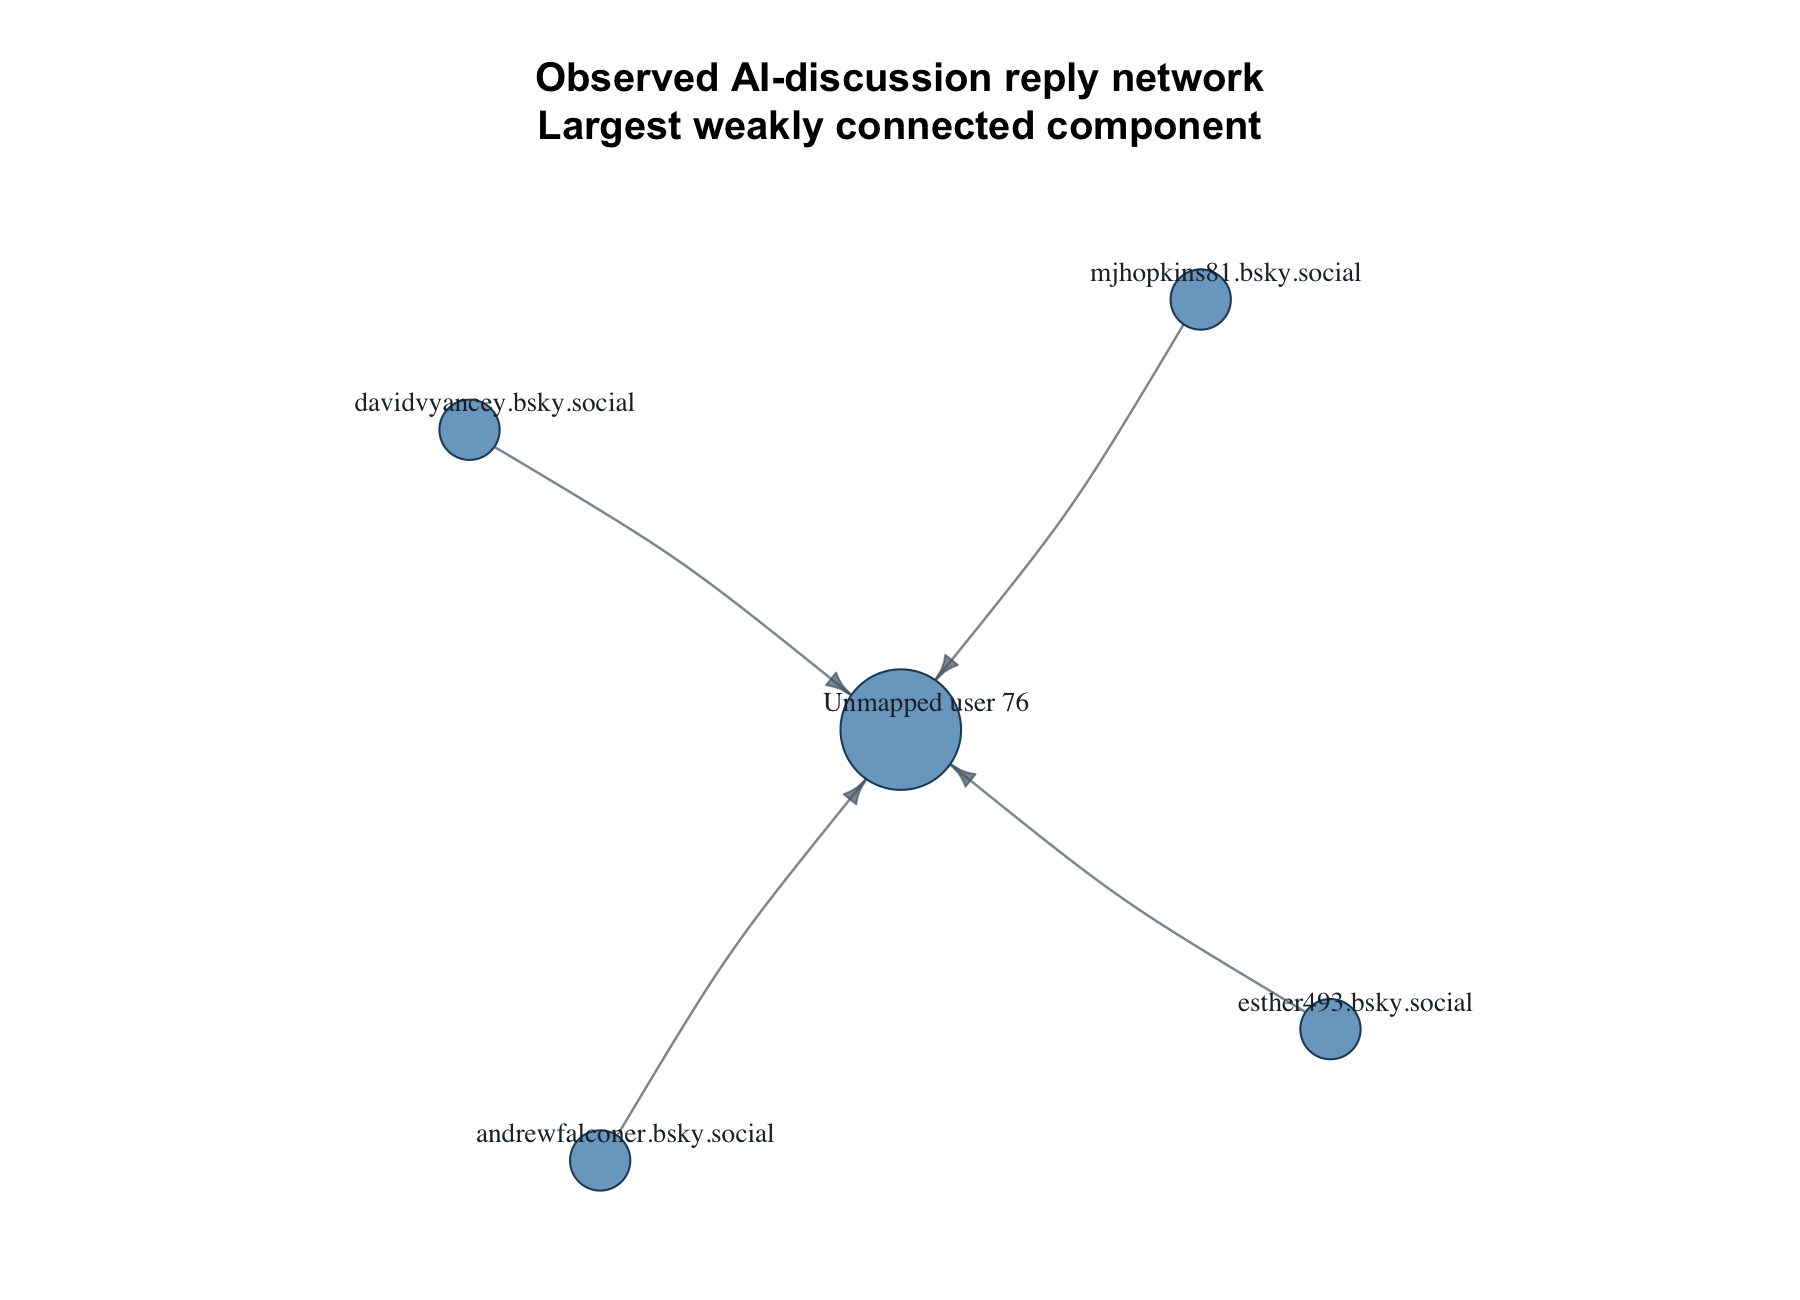
\includegraphics[width=0.94\linewidth]{../figures/rq3_reply_network} 

}

\caption{Figure 5. The largest weakly connected component of the observed reply network. Arrows run from reply author to parent-post author; node size represents weighted directed PageRank. Only 5 of 240 edge-connected users appear in this figure.}\label{fig:rq3-network-figure}
\end{figure}

The largest component is a four-to-one reply pattern: four sampled reply
authors each replied to the same target. The central target consequently
has the highest in-degree (4) and PageRank in the observed network. Its
handle was unavailable because the parent post fell outside the
collected search results, so the figure uses a safe ``Unmapped user''
label. This position indicates centrality only in the sampled reply
network, not global influence on Bluesky.

Of the 240 network users, 128 mapped unambiguously to handles and 112
did not. Every unmapped user was a target-only parent-post author whose
original post was outside the collection. Community detection was
omitted because partitioning 111 tiny disconnected components would
offer little defensible substantive interpretation.

\textbf{RQ3 answer.} Sampled reply activity was sparse and highly
fragmented. Most interactions occurred in isolated pairs or very small
components rather than a cohesive discussion network.

\section{Integrated Discussion}\label{integrated-discussion}

The three analyses describe different layers of the same sampled
discourse. RQ1 shows genuine topical and stylistic variety, but the weak
separation and uneven cluster sizes caution against describing seven
natural topics. Three broader substantive themes are more stable than
the full seven-cluster partition.

RQ2 indicates that engagement is not distributed identically across
those lexical patterns, yet the small epsilon-squared shows that cluster
membership explains little rank variation. Extreme posts, zero-heavy
outcomes and the very small Cluster 5 all matter to interpretation.
Statistical significance should not be confused with a large practical
difference.

RQ3 adds a structural distinction: topical variety and post-level
engagement did not translate into one interconnected sampled
conversation. The reply graph consists almost entirely of pairs and tiny
components. A highly engaged post or higher-engagement lexical cluster
is not necessarily associated with a user occupying a bridging network
position; indeed, no such brokerage position exists in this edge sample.

Together, the results portray a heterogeneous but dispersed sample of
AI-related Bluesky activity: varied language and content, modest
engagement differences, and fragmented reply relationships. These
conclusions apply to the collected posts, not Bluesky as a whole.

\section{Limitations}\label{limitations}

\begin{enumerate}
\def\labelenumi{\arabic{enumi}.}
\tightlist
\item
  \textbf{Search-term sampling.} Four keywords cannot capture all
  AI-related discussion, and the results are not platform-wide
  estimates.
\item
  \textbf{Variable pilot relevance.} Manual relevance ranged from 68\%
  to 88\%, indicating keyword-dependent noise and coverage.
\item
  \textbf{Repeated and syndicated content.} Exact duplicates were
  controlled during clustering and restored carefully for post-level
  engagement, but near-duplicate news and templates still influenced
  smaller clusters.
\item
  \textbf{Weak cluster separation.} Only about 6.84\% of TF-IDF
  variation lay between clusters; the seven groups are descriptive, not
  natural boundaries.
\item
  \textbf{Representation choices.} Unigram TF-IDF and primarily English
  stopwords may underrepresent phrases, multilingual meaning and
  contextual nuance.
\item
  \textbf{Engagement distribution.} Engagement was zero-heavy,
  right-skewed and influenced by extreme observations.
\item
  \textbf{Small Cluster 5.} Its median of 3 is based on only 13 posts
  and should not be generalised into a broad claim about AI-art
  engagement.
\item
  \textbf{Incomplete reply graph.} The network contains only reply
  relationships observable from collected posts, not followers,
  friendships, endorsements or the complete Bluesky graph.
\item
  \textbf{Edge-list scope.} Authors without an observed reply
  relationship are absent from the 240-user network.
\item
  \textbf{Unmapped targets.} The 112 unmapped users were target-only
  authors of parent posts outside the search sample; they were retained
  but not identified speculatively.
\item
  \textbf{Observational design.} All findings are descriptive
  associations and support no causal conclusion.
\end{enumerate}

\section{Conclusion}\label{conclusion}

AI-related posts in this Bluesky sample formed seven reproducible but
weakly separated lexical clusters. Inspection supported roughly three
broader substantive themes, while smaller clusters often reflected
syndication, employment templates, language patterns or event-specific
reporting.

Engagement differed significantly across the seven clusters, H(6) =
35.12, p \textless{} .001, but the effect was small (epsilon-squared =
0.032) and remained similar after excluding repeated-text posts. The
observed reply network was even more qualified: 240 connected users
separated into 111 weak components, with only 5 users in the largest.

The coherent finding is therefore one of \textbf{diversity without
cohesion}: the sample contains varied AI discourse and modest engagement
differences, but reply interactions remain dispersed across many small
conversations.

\section{References}\label{references}

No external literature is cited in this report. Data definitions,
transformations and analytical procedures are documented in the
repository README, scripts 01--05 and generated outputs. Package
implementations used by the workflow include \texttt{bskyr},
\texttt{dplyr}, \texttt{ggplot2}, \texttt{igraph}, \texttt{knitr} and
\texttt{rmarkdown}. No publication details or URLs have been added
without repository support.

\section{Reproducibility Appendix}\label{reproducibility-appendix}

The report reads completed outputs rather than rerunning data
collection, clustering, hypothesis testing or network analysis. The
pipeline is implemented in numerical order:

\begin{Shaded}
\begin{Highlighting}[]
\NormalTok{scripts/01\_data\_collection.R}
\NormalTok{scripts/02\_text\_analysis.R}
\NormalTok{scripts/03\_clustering.R}
\NormalTok{scripts/04\_hypothesis\_testing.R}
\NormalTok{scripts/05\_network\_analysis.R}
\end{Highlighting}
\end{Shaded}

The stored canonical raw dataset permits reproduction without new API
requests. Randomised clustering and network layout use fixed seeds,
while RQ2 tests are deterministic.

View R session information

\begin{verbatim}
## R version 4.5.2 (2025-10-31)
## Platform: aarch64-apple-darwin20
## Running under: macOS Tahoe 26.6.2
## 
## Matrix products: default
## BLAS:   /System/Library/Frameworks/Accelerate.framework/Versions/A/Frameworks/vecLib.framework/Versions/A/libBLAS.dylib 
## LAPACK: /Library/Frameworks/R.framework/Versions/4.5-arm64/Resources/lib/libRlapack.dylib;  LAPACK version 3.12.1
## 
## locale:
## [1] en_US.UTF-8/en_US.UTF-8/en_US.UTF-8/C/en_US.UTF-8/en_US.UTF-8
## 
## time zone: Australia/Sydney
## tzcode source: internal
## 
## attached base packages:
## [1] stats     graphics  grDevices utils     datasets  methods   base     
## 
## other attached packages:
## [1] dplyr_1.2.1
## 
## loaded via a namespace (and not attached):
##  [1] digest_0.6.39     R6_2.6.1          fastmap_1.2.0     tidyselect_1.2.1 
##  [5] xfun_0.56         magrittr_2.0.4    glue_1.8.0        tibble_3.3.1     
##  [9] knitr_1.51        pkgconfig_2.0.3   htmltools_0.5.9   rmarkdown_2.31   
## [13] generics_0.1.4    lifecycle_1.0.5   cli_3.6.5         vctrs_0.7.1      
## [17] withr_3.0.2       compiler_4.5.2    rstudioapi_0.18.0 tools_4.5.2      
## [21] pillar_1.11.1     evaluate_1.0.5    yaml_2.3.12       rlang_1.3.0
\end{verbatim}

\end{document}
